%--------------------------------------------------------------------------------------------------%
\chapter{PENDAHULUAN}
\label{chap:1}
%--------------------------------------------------------------------------------------------------%

%--------------------------------------------------------------------------------------------------%
\section{Latar Belakang}
\label{sec:latar-belakang}
%--------------------------------------------------------------------------------------------------%

\Legal adalah peraturan tertulis yang memuat norma hukum yang mengikat secara umum dan dibentuk atau
ditetapkan oleh lembaga negara atau pejabat yang berwenang melalui prosedur yang ditetapkan dalam
\legal, sesuai yang dijelaskan dalam Undang-Undang Republik Indonesia Nomor 12 Tahun 2011
(selanjutnya disebut dengan UU 12/2011). \Legal dapat digunakan untuk menjawab pertanyaan-pertanyaan
yang berkaitan dengan hukum, seperti:

\begin{itemize}
  \item Peraturan apa yang berlaku pada daerah X yang disahkan di tahun Y?
  \item Apa relasi suatu peraturan dengan peraturan lain?
  \item Mana saja peraturan yang membahas tentang topik W atau X tapi bukan topik Y dan bukan Z?
  \item Apa isi dari Pasal X ayat (Y) huruf Z dari suatu \legal?
  \item Apa saja bab-bab yang terdapat pada peraturan X?
\end{itemize}

Pertanyaan-pertanyaan tersebut umumnya biasa dijawab oleh seorang ahli hukum, yang hanya dapat
dilakukan dalam skala kecil dan biaya relatif mahal. Komputer dapat menjadi alternatif untuk
aplikasi tersebut dalam skala lebih besar dan biaya lebih murah, jika \legal berupa data terstruktur
yang dapat diolah oleh komputer. Saat ini pembuatan dan pemanfaatan \legal masih dilakukan secara
manual oleh manusia. Pembuatan \legal dilakukan dengan mengetikkan konten peraturan tersebut dengan
format yang telah ditentukan. Metode pembuatan tersebut tidak masalah jika hanya akan dibaca oleh
manusia karena manusia secara tidak sadar dapat melihat hirarki visual dari dokumen tersebut dan
membuat data yang dilihatnya terstruktur di dalam otak. Metode ini membuat pemanfaatan \legal oleh
mesin menjadi kurang efisien karena mesin perlu melakukan proses tambahan yaitu mengonversi gambar
menjadi data terstruktur.

\begin{figure}[H]
  \centering
  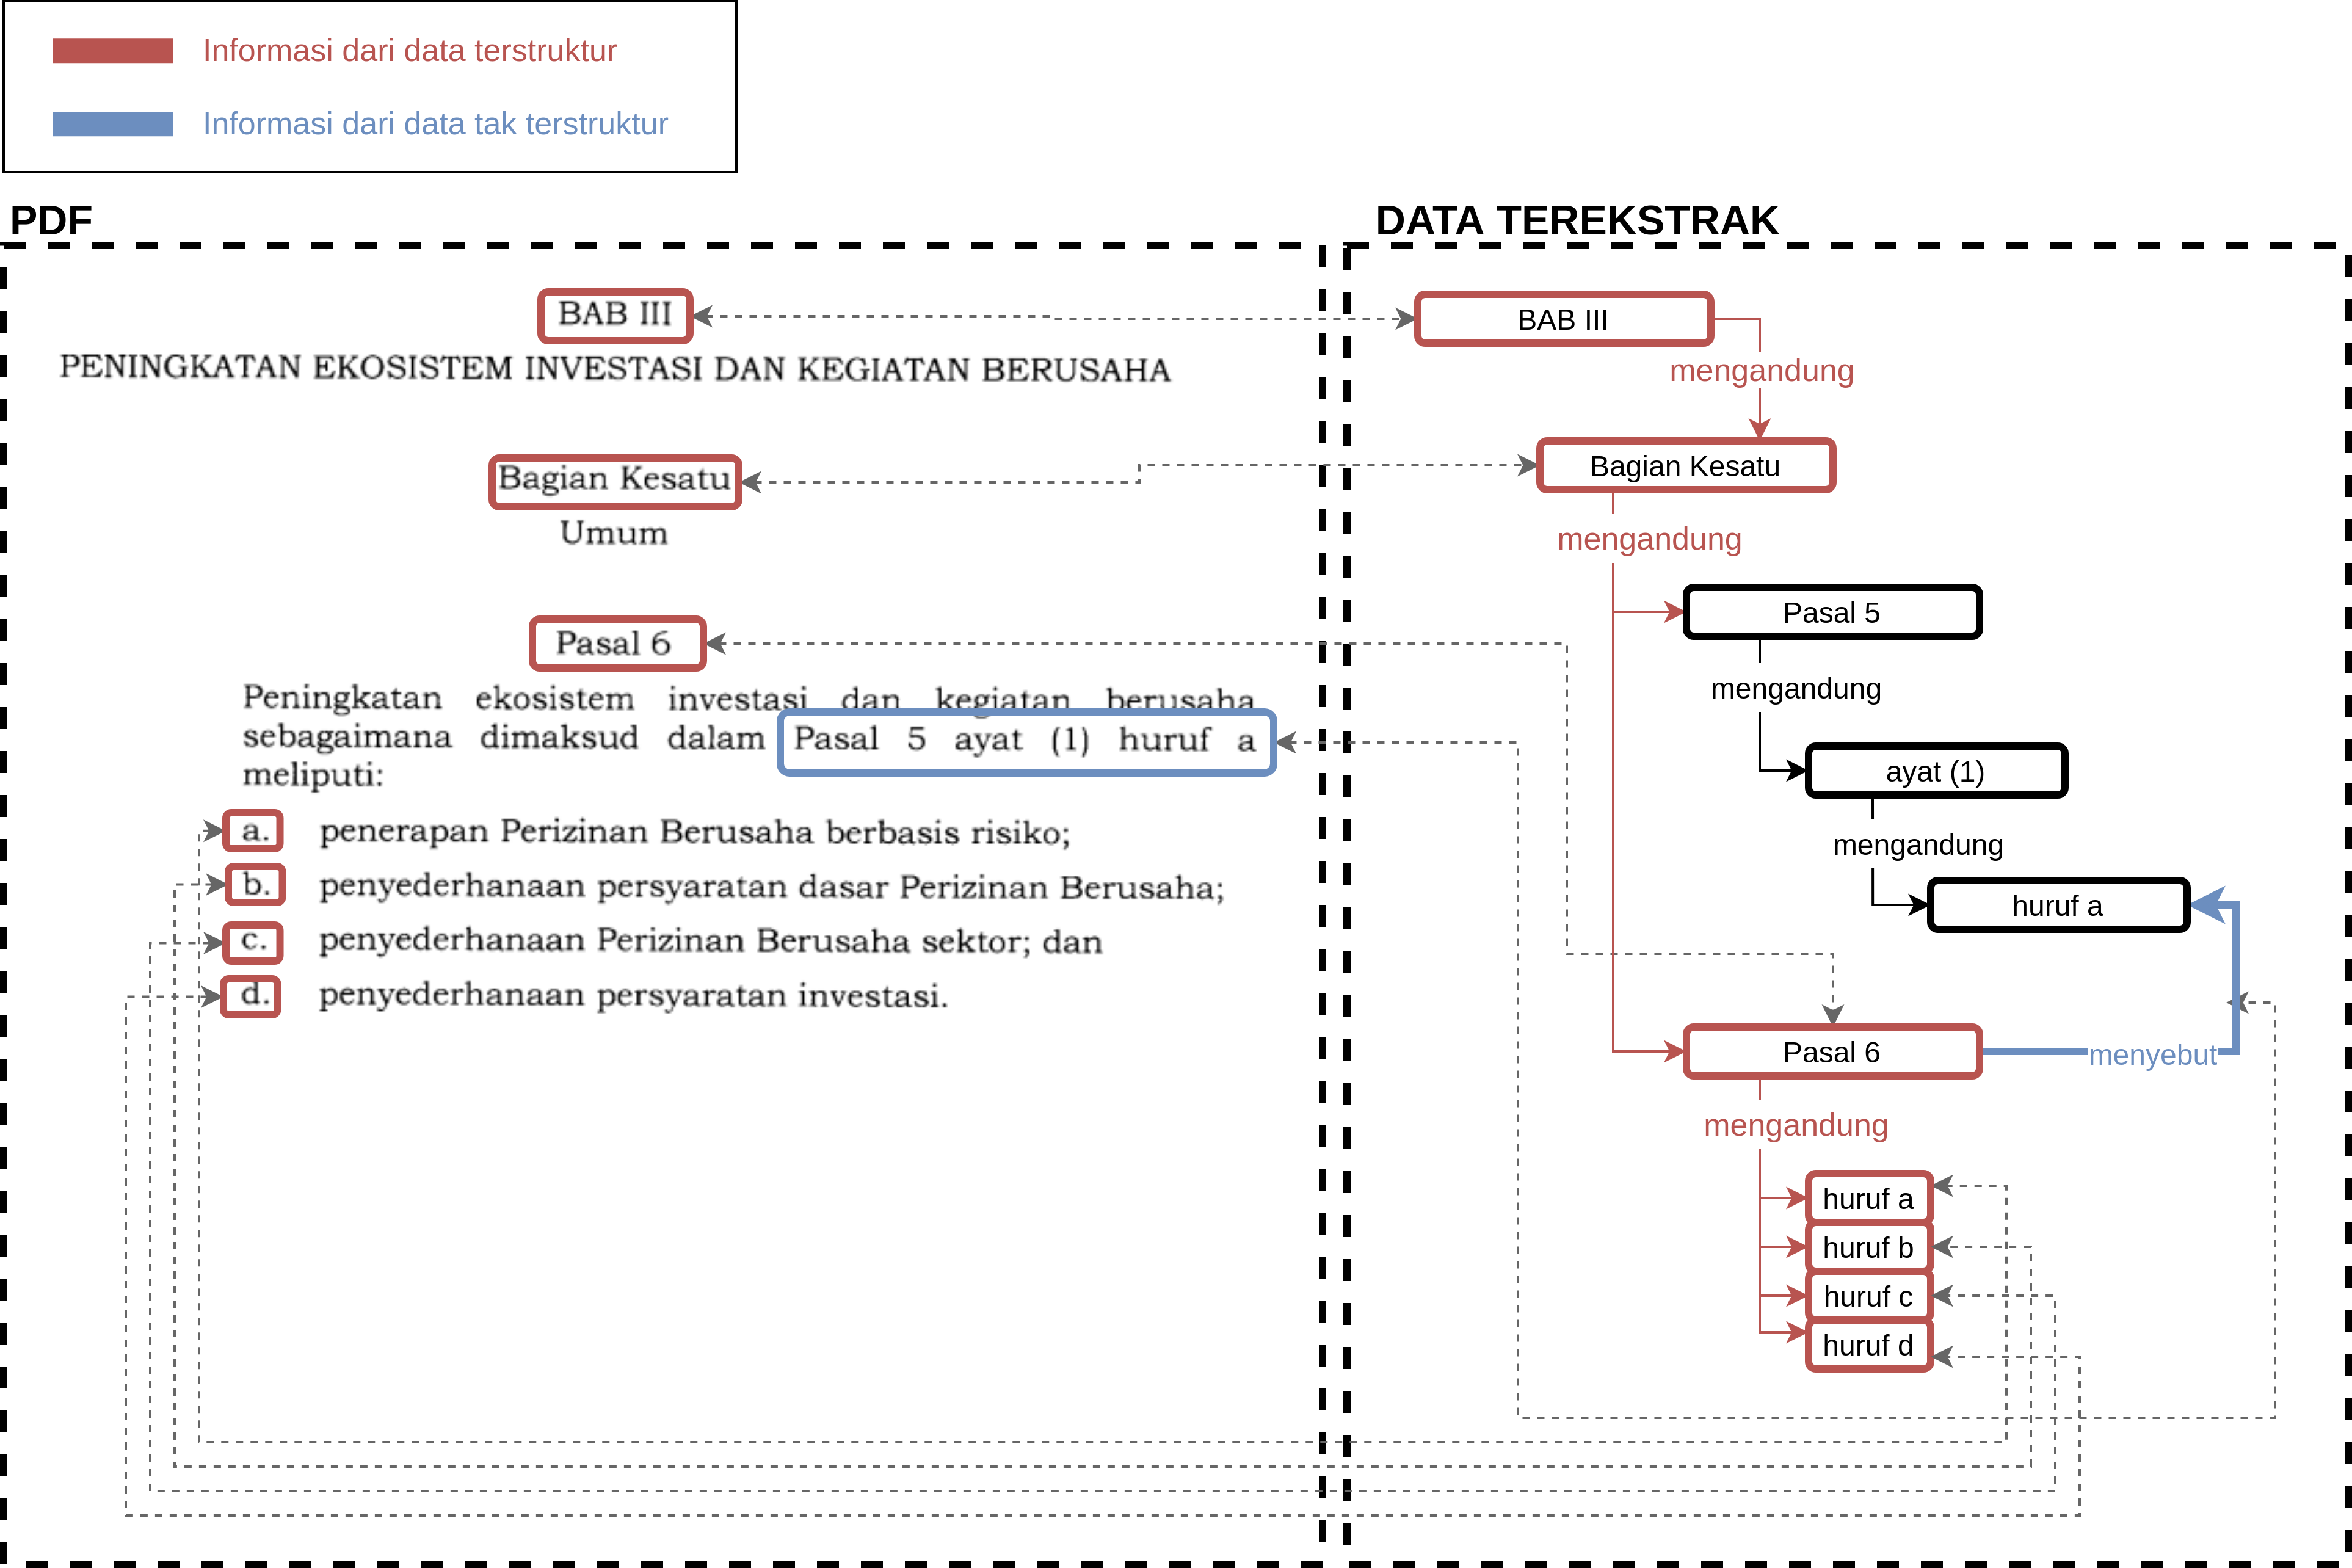
\includegraphics[width=\textwidth]{pictures/terstruktur.png}
  \caption{Cuplikan ekstraksi data terstruktur dan data tidak terstruktur dari dokumen PDF UU 11/2020 tentang Cipta Kerja}
  \label{fig:ekstraksi-dokumen}
\end{figure}

\pic~\ref{fig:ekstraksi-dokumen} menampilkan contoh ekstraksi informasi dari UU 11/2020 tentang
Cipta Kerja. Pada gambar tersebut terlihat bahwa terdapat dua jenis ekstraksi data yaitu ekstraksi
dari data terstruktur (merah) dan ekstraksi dari data tidak terstruktur (biru). Contoh data
terstruktur pada dokumen tersebut adalah \textit{section} pada dokumen seperti \textbf{Bab III},
\textbf{Bagian Kesatu}, \textbf{Pasal 6}, dan \textbf{huruf a - d}. Contoh data tidak terstruktur
pada dokumen tersebut adalah semua teks yang terdapat pada \textit{section} tersebut seperti teks
``penerapan Perizinan Berusaha berbasis risiko;'' yang terdapat pada \textbf{huruf a}. Manusia perlu
membaca manual untuk mengetahui bahwa UU 11/2020 mengandung \textbf{Bab III}, \textbf{Bab III}
mengandung \textbf{Bagian Kesatu}, \textbf{Bagian Kesatu} mengandung \textbf{Pasal 6}, dan
\textbf{Pasal 6} mengandung \textbf{huruf a - d}. Pada gambar tersebut, dalam mengekstraksi
informasi ``UU 11/2020 Pasal 6 merujuk kepada Pasal 5 ayat (1) huruf a'', manusia pertama-tama perlu
membaca dari awal teks pasal-pasal pada UU perujukan (citation), dan kemudian meng-\textit{infer}
informasi lengkap berdasarkan konteks \legal.

\begin{figure}[H]
  \centering
  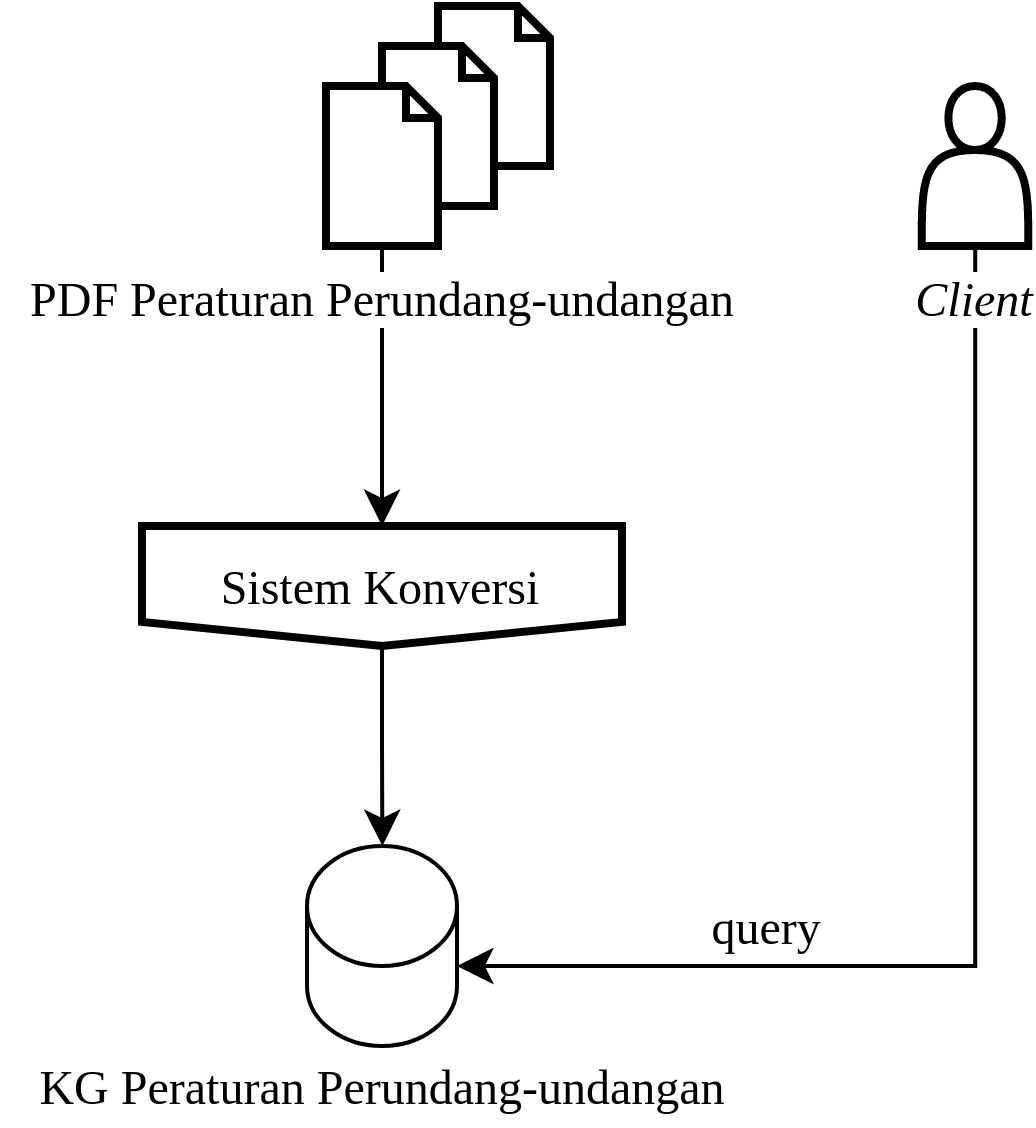
\includegraphics[scale=0.25]{pictures/konstruksi-dan-query.png}
  \caption{Bagan alir pembuatan dan \textit{query} KG \legal}
  \label{fig:konstruksi-dan-query}
\end{figure}

Data terstruktur yang digunakan dapat dalam berbagai format seperti JSON, XML, CSV, maupun skema
basis data SQL. Menurut \textit{5-star deployment scheme for Open
Data},\footnote{\url{https://5stardata.info/en/}} jenis data dapat dikategorikan menjadi 5 tingkat
yaitu \textit{1-star} hingga \textit{5-star}. \textit{5-star data} merupakan data dengan jenis
informasi paling bermanfaat, memberikan data dalam bentuk \textit{open license}, terstruktur,
tersedia dalam \textit{open format}, menggunakan URI sebagai notasi data, dan dapat dihubungkan
(\textit{linked}) dengan data lain. Pada penelitian ini penulis menggunakan \textit{Knowledge Graph}
sebagai struktur data hasil ekstraksi perundang-undangan, yang mana terkategori sebagai
\textit{5-star}. \textit{Knowledge graph} (KG) adalah struktur data yang (i) menggambarkan entitas
dunia nyata dan keterkaitannya, tersusun dalam bentuk \textit{graph}, (ii) mendefinisikan kelas
entitas dan relasi antar entitas dalam bentuk skema, (iii) membolehkan sembarang entitas memiliki
relasi satu sama lain dan (iv) mencakup berbagai topik domain \citep{paulheim_2016}. Dengan
melakukan ekstraksi data dari dokumen yang bersifat semi-terstruktur, \legal dapat dikonversi
menjadi KG. Sebagai manfaatnya, dapat fitur-fitur berbasis \textit{query} seperti \textit{question
answering}, \textit{reasoning} dan visualisasi data. \pic~\ref{fig:konstruksi-dan-query} menampilkan
garis besar dari peneilitan ini yaitu konstruksi KG \legal serta pemanfaatannya dari KG \legal
tersebut dalam yang dapat dilakukan dengan melakukan \textit{query}.

Untuk melakukan konversi dari PDF menjadi KG, secara umum dibutuhkan pemahaman struktur PDF tersebut
sehingga dapat dilakukan \textit{parsing} menjadi data yang dapat diproses oleh komputer, kemudian
dibutuhkan juga \textit{vocabulary} untuk menentukan KG seperti apa yang ingin dibuat. Spesifik pada
kasus \legal ini, penulis perlu mengetahui struktur serta konteks dari PDF peraturan
perundang-undangan, kemudian memerlukan \textit{vocabulary} spesifik untuk \legal yang menjadi dasar
pembuatan KG. Beberapa usaha telah dilakukan untuk membuat \textit{vocabulary} untuk KG \legal
seperti ELI,\footnote{\url{https://eur-lex.europa.eu/eli-register/about.html}}
Schema.org,\footnote{\url{https://schema.org}} dan
Wikidata.\footnote{\url{https://www.wikidata.org}}


\begin{listing}[H]
  \begin{minted}[fontsize=\scriptsize, frame=single, breaklines]{turtle}
@prefix schema: <http://schema.org/> .
@prefix xsd: <http://www.w3.org/2001/XMLSchema#> .

<http://data.europa.eu/eli/dir/1980/181/oj> a schema:Legislation ;
  schema:about <http://eurovoc.europa.eu/1896> ;
  schema:isBasedOn <http://njh.me/11957E100.html> ;
  schema:legislationDate "1979-12-20"^^schema:Date ;
  schema:legislationPassedBy "Council of the European Union"^^xsd:string ;
  schema:name "Council Directive 80/181/EEC of 20 December 1979 on the approximation of the laws of the Member States relating to units of measurement and on the repeal of Directive 71/354/EEC"^^xsd:string ;

<http://eurovoc.europa.eu/1896> a schema:Thing ;
  schema:name "Metrology"^^xsd:string .

<http://njh.me/11957E100.html> a schema:Legislation .
  \end{minted}
  \caption{Contoh KG metadata dokumen legal menggunakan \textit{vocabulary} Schema.org}
  \label{lst:schema-org-example}
\end{listing}

Pada \lst~\ref{lst:schema-org-example} diberikan contoh KG yang dibuat dengan \textit{vocabulary}
Schema.org. Contoh KG tersebut memuat metadata peraturan seperti tentang apa peraturan tersebut
(\code{schema:about}), apa dasar dari peraturan tersebut (\code{schema:isBasedOn}), dan nama dari
peraturan tersebut (\code{schema:name}). Akan tetapi, baik Schema.org maupun vocabulary-vocabulary
lainnya seperti pada ELI dan Wikidata, tidak dapat merepresentasikan struktur beserta isi peraturan.
Selain itu, \textit{vocabulary} tersebut dirancang secara generik, sehingga tidak dapat
merepresentasikan data yang secara spesifik terdapat pada \legal di Indonesia. Sehingga dengan
membuat \textit{vocabulary} untuk \legal di Indonesia, diharapkan dapat menjadi kontribusi dalam
memperluas penggunakan data struktur, terutama KG, dalam pembuatan dan pemeliharaan dokumen \legal.

Lex2KG merupakan \textit{framework} yang dikembangkan pada penelitian ini, dapat mengonversi dokumen
menjadi KG secara otomatis. Lex diambil dari Bahasa Latin yang artinya hukum, atau \textit{legal}
dalam Bahasa Inggris. Belum ada pekerjaan terkait yang melakukan automasi konversi dokumen \legal
menjadi KG secara otomatis. Oleh karena itu Lex2KG diharapkan dapat menjadi kontribusi yang
mendukung pembuatan dan penggunaan KG secara umum, dan bidang hukum secara khusus. Diluar dari
contoh \textit{use case} yang dijelaskan pada tulisan ini, KG yang dibuat oleh Lex2KG dapat
dikembangkan lebih lanjut dengan menggunakan kelebihan KG yaitu kemudahan untuk mengaitkan KG.
Sebagai contoh, data pada KG tentang peraturan dengan topik penyakit dapat dihubungkan dengan KG
penyakit untuk dapat dilakukan pencarian dalam pengetahuan yang lebih luas.

%--------------------------------------------------------------------------------------------------%
\section{Permasalahan}
\label{sec:permasalahan}
%--------------------------------------------------------------------------------------------------%

Berikut adalah rumusan permasalahan dari penelitian yang dilakukan:
\begin{itemize}
  \item Bagaimana membuat ontologi agar KG yang dihasilkan dapat menjawab \textit{competency questions}?
  \item Bagaimana merancang suatu sistem untuk melakukan konversi otomatis PDF \legal menjadi KG
        berdasarkan ontologi yang sudah dibuat?
  \item Bagaimana hasil konversi dan evaluasi terhadap KG \legal tersebut?
\end{itemize}

%--------------------------------------------------------------------------------------------------%
\section{Batasan Permasalahan}
\label{sec:batasan-permasalahan}
%--------------------------------------------------------------------------------------------------%

Berikut adalah batasan dari penelitian yang dilakukan:
\begin{itemize}
  \item Konversi hanya dapat dilakukan pada \legal di Indonesia
  \item Peraturan yang di-\textit{maintain} kualitas konversinya dibatasi kepada beberapa peraturan
        UU dan non-UU dengan format PDF yang sama dengan PDF yang diperoleh dari Laman Undang-Undang Jaringan
Dokumentasi dan Informasi Hukum DPR RI.
  \item Peraturan yang di-\textit{maintain} kualitas konversinya memiliki jumlah yang
        \textit{imbalanced} untuk UU dan peraturan jenis lainnya
  \item Tidak dapat melakukan \textit{query} terhadap KG yang kompleks seperti \textit{query} yang
        membutuhkan \textit{natural language processing} (contoh: ``Jika saya berusia 12 tahun,
        apakah saya boleh bekerja menurut UU Ketenagakerjaan?'') atau yang membutuhkan konteks
        semantik seperti \textit{abnormality/consistency detection}.
\end{itemize}

%--------------------------------------------------------------------------------------------------%
\section{Metodologi Penelitian}
\label{sec:metodologi-penelitian}
%--------------------------------------------------------------------------------------------------%

Metodologi penelitian dilakukan sesuai dengan yang diilustrasikan pada \pic~\ref{fig:metodologi}.
Perancangan sebuah KG dimulai dengan membuat \textit{competency questions}.


\begin{figure}
  \centering
  \begin{tikzpicture}[node distance=0.5cm]
    %Styles   
    \tikzstyle{r} = [rectangle, minimum width=7cm, minimum height=0.5cm, draw, text centered]

    %Nodes
    \node[r] (pertanyaan)                           {Merancang \textit{Competency Questions}};
    \node[r] (ontologi)     [below=of pertanyaan]   {Perancangan Ontologi};
    \node[r] (pengembangan) [below=of ontologi]     {Pengembangan Sistem Konversi};
    \node[r] (usecase)      [below=of pengembangan] {\textit{Use Case Evaluation}};

    %Lines
    \draw[->] (pertanyaan.south)   -- (ontologi.north);
    \draw[->] (ontologi.south)     -- (pengembangan.north);
    \draw[->] (pengembangan.south) -- (usecase.north);

  \end{tikzpicture}
  \caption{Metodologi Penelitian}
  \label{fig:metodologi}
\end{figure}

Setelah merancang \textit{competency questions}, penelitian dilenjutkan dengan merancang ontologi
(desain KG) yang dapat menjawab \textit{competency questions} tersebut. Ontologi ini kemudian akan
digunakan sebagai landasan sistem konstruksi KG. Karena sulit untuk menjamin hasil konversi untuk
semua PDF \legal, akan terdapat beberapa PDF yang akan di-\textit{maintain} kualitas konversinya
yang selanjutnya akan disebut \textit{maintained PDFs}. Pengembangan sistem konversi dilakukan
secara iteratif. Setiap terjadi perubahan pada sistem konversi, akan diperiksa apakah untuk semua
\textit{maintained PDFs} memberikan hasil konversi dengan kualitas yang tinggi. Sistem konversi akan
menerima input berupa PDF dan mengeluarkan output berupa KG dengan ontologi yang sudah dirancang
pada tahap sebelumnya.

Untuk menjamin KG yang dibuat dapat menjawab \textit{competency questions}, dalam penelitian ini
dilakukan \textit{use case evaluation} yaitu berupa demonstrasi contoh penerapan dari KG berdasarkan
\textit{competency questions}. Setelah semua \textit{competency questions} dapat terjawab oleh KG
dari \textit{maintained PDFs} dan dilakukan \textit{use case evaluation}, dilakukan \textit{large
scale evaluation} di mana PDF di luar \textit{maintained PDFs} akan dikonversi kemudian dilakukan
sampling pada hasil konversinya untuk dievaluasi secara kualitatif.

%--------------------------------------------------------------------------------------------------%
\section{Sistematika Penulisan}
\label{sec:sistematika-penulisan}
%--------------------------------------------------------------------------------------------------%

Penelitian ini dibagi ke dalam 6 bab bahasan. Bab pertama menjelaskan mengenai pendahuluan yang
berisikan latar belakang serta konteks penelitian yang dilakukan. Pada bab kedua dijelaskan mengenai
tinjauan pustaka yang dilakukan di mana dijelaskan berbagai istilah dan bidang ilmu yang berkaitan
dengan penelitian yang dilakukan. Lalu, pada bab ketiga dijelaskan mengenai perancangan penelitian
yang dilakukan dalam menyusun penelitian ini. Selanjutnya, bab keempat akan membahas implementasi
penelitian. Bab kelima akan membahas evaluasi dan analisis hasil penelitian. Bab keenam akan
membahas kesimpulan penelitian dan saran untuk penelitan selanjutnya.